\chapter{Object~Detection}
\label{chap:object_detection} 


\section{Introduction}


\section {Image preparation}

One thing which was noticed in the implementation of the segmentation tool from chapter \ref{chap:bootstrap} was that the original images were often much clearer than the scaled down images for a human annotator to see fine details.

With that in mind I focused on preserving resolution for the annotation process. There may be other reasons to prefer smaller images, such as faster training or inference (which we explore below in section \ref{sec:crop_size}, faster loading, reduced memory size, or reduce disk space. 

The additional benefit to preserving resolution is that performance of a given object detector has generally been shown to be better with higher image resolution, when training on data with a limited number of classes, we hypothesis that it is possible to get away with larger image sizes by using much smaller crops of the original images to train, as long as the objects fit in the image crops. We do some experiments on this idea in \ref{sec:crop_size}.

As a counter example the images in the PASCAL VOC \cite{Everingham2008}, or COCO\cite{Lin2014} datasets have a large range of scales, where many large objects which occupy almost the entirety of the image. For the majority of data experimented on in this thesis, the objects of interest occupy an area much smaller than the whole image size. An analysis of the object sizes in the datasets can be seen in figure \ref{fig:box_sizes}.


\todo{box sizes analysis figure}

\begin{figure}[ht]
\centering
%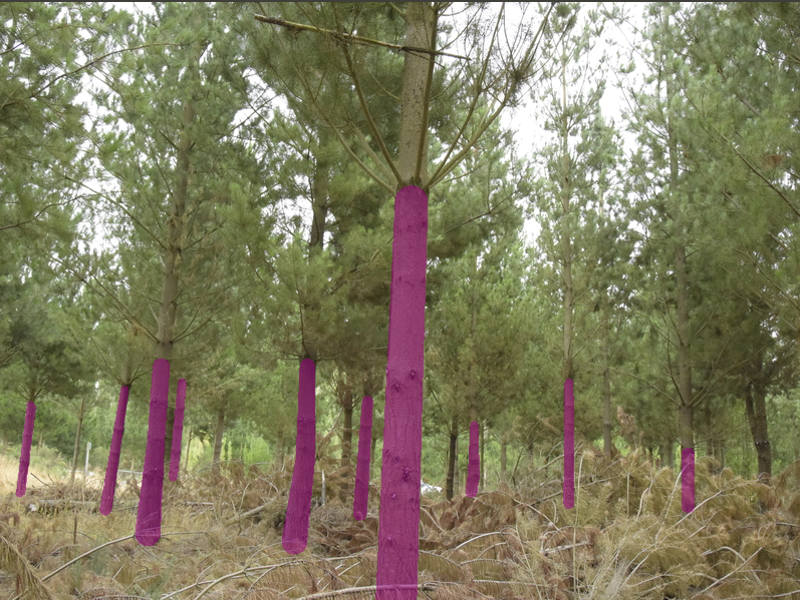
\includegraphics[width=0.9\linewidth]{bootstrap/trees_example.png}

\caption{Object bounding box sizes}
\label{fig:box_sizes}
\end{figure}


Use of simpler, faster models has been successful as the backbone of the object detection network (for example ResNet--18), which enables larger images in both training and evaluation. Time taken for evaluation and training is also much improved relative to using larger networks. For the smaller datasets in our experiments I did not see large improvements in accuracy when using larger backbone networks.

\begin{table}[h]
  \centering
    \caption{Ranges of parameters used for image augmentation, translation occurs as part of a cropping process}
    
  \begin{tabular}{ l  l }
    Parameter & Range \\
    \toprule
    scale (log uniform) & ${3/4}$--${4/3}$  \\ 
    aspect scale  & $ 1 \pm 0.1 $  \\ 

    brightness adjustment (additive) & $ \pm 10 $ \\ 
    contrast (multiplicative) & $ 1 \pm 0.1 $ \\ 

    gamma adjustment & $ \pm 0.1 $ \\ 

    hue shift & $ \pm 5 $ \\ 
    saturation shift & $ \pm 5 $ \\ 
    
    horizontal flips & $ P = 0.5 $ \\ 
    
    \bottomrule
  \end{tabular}
\label{fig:obj_augmentation}
\end{table}

After applying augmentation (photo-metric distortion and scaling) with parameters described in table \ref{fig:obj_augmentation} and image whitening (described below), a region is cropped from the resulting image at random. In the case where the crop region is larger than the input image, an image is created with pixels set to zero and the input image is placed at a random position within the image.

The crop sizes are $600\times600$ unless otherwise specified, for example the tree branch detection uses $300\times300$ due to smaller input images.


We employ image whitening to ensure consistency with ImageNet trained models (used as the backbone of the networks) subtracting mean (r, g, b) $ (0.485. 0.456, 0.406) $ and dividing by standard deviation $ (0.229, 0.224, 0.225) $.


\section {Object detection}

The object detection method I have been using for the following experiments is a modified RetinaNet \cite{Lin2017} as a strong near-state of the art object detector and having a simple implementation as a single stage object detection method. 


\subsection {Network architecture}
\label{sec:architecture}


Some parameters and network architectures differ from the original paper. For the most part the modifications are small things which seem to enable it to learn better on the kind of small datasets I experiment with below. 

These include adding extra residual layers to the decoder, shown in figure \ref{fig:detection_network}. It is more similar to the network shown in  \ref{chap:bootstrap} than the \gls{FCN} network. A key difference is that the weights between class subnets nor box subnets are shared (the original shares weights between class subnets), as it was found it to slow down initial training considerably. 


Other differences are necessary to accommodate different box sizes (usually using additional finer layer(s) of anchor boxes to handle small objects).


\subsection {Object detection loss}

The complete loss function is a combination of classification loss, and bounding box regression loss.


\subsection{Anchor boxes}

I use a set of anchors boxes for each level with aspect ratios $ \in \{0.5, 1, 2\} $ and scales $ \in \{2^0, 2^{1/3}, 2^{2/3}\} $. For each feature map at level $k$, with a base scale of $ 2^{k + 2} $ pixels, the set of 9 anchor boxes (all combinations of aspect and scale) are tiled centred on each pixel. 

In the case of counting, where circles are used for annotation only three anchor boxes are used, only the square aspect ratio is used at the same three scales. For all intents and purposes the circles with radius $r$ are treated as a square box with side lengths $2r$, and the box regression sub-network modified to produce only $3$ outputs (enforcing square aspect ratio for height and width).

Feature maps on levels $3$--$7$ are used for most datasets giving the smallest (square) anchor at $32\times32$ and the largest at $812\times812$ 

For those with smaller objects such as the aerial Adellie penguin counting, the tree branch detection and the seal counting an extra feature map is used giving anchor boxes as small as $16\times16$ and more densely tiled.

In training, anchor boxes are selected by matching on \gls{IOU} overlap with ground truth boxes. Each anchor is matched with the ground truth box with highest overlap. An anchor box matches a ground truth box as a positive if the IOU $ overlap >= 0.5 $, anchors with IOU $ overlap < 0.4 $ are treated as negative, and those boxes with $ 0.5 > overlap >= 0.4 $ are ignored (omitted from either positive or negative for computing loss).

Ground truth boxes will match with potentially many anchor boxes, but those in close proximity and similar size may mean that boxes which would have otherwise matched do not, because anchors cannot be assigned to more than one ground truth.

\subsection {Box regression loss}


We use the anchor box encoding used in \gls{RCNN} \cite{Wang2017} for the purpose of calculating location loss. The loss is a smooth-L1 loss over four regression targets ($t_x, t_y, t_w, t_h$) giving a transformation from an anchor box ($a_x, a_y, a_w, a_h$)  to a target box from the ground truth ($g_x, g_y, g_w, g_h$). 

The boxes are encoded as the offset of the centre in both directions (in proportion to the box size) and the log scale of height and width. The encoding of the four targets are given as:

\begin{equation}
\begin{split}
t_x = (g_x - a_x) a_w\\
t_y = (g_y - a_y) a_h\\
t_w = log(g_w / a_w)\\
t_h = log(g_h / a_h)\\
\end{split}
\label{eq:encoding_rcnn}
\end{equation}

The localisation loss can be directly computed from these targets and the output of the box prediction sub-network as the sum of the 4 smooth-L1 regressions. Smooth-L1 is a combination of L2 loss near the origin and L1 loss otherwise. It is given as:

\begin{equation}
L_{1;smooth} = 
\begin{cases*}
|x| & if $|x|>\alpha $ \\
\frac{1}{|\alpha|}x^2 & if $|x| \leq \alpha$
\end{cases*}
\label{eq:smooth_l1}
\end{equation}

The commonly used value $\alpha = 0.5$ is used here.

By rearranging the equations we can then do the reverse process and decode bounding boxes from box prediction targets and an anchor box. Here I substitute $ g $ for $ p $ to denote a bounding box prediction instead of a ground truth.

\begin{equation}
\begin{split}
p_x = a_x + t_x  a_w\\
p_y = a_y + t_y  a_h\\
p_w = exp(t_w) a_w \\
p_h = exp(t_h) a_h\\
\end{split}
\label{eq:encoding_rcnn}
\end{equation}

\subsection {Focal loss}
\label{sec:loss}


The experiments use a modified version of the Focal Loss \cite{Lin2017} to handle the class imbalance (negative vs. positive) present when sampling anchor box predictions densely.

Focal Loss \cite{Lin2017} re-weights the standard \gls{BCE} loss function to deal with a large number of easy negative examples in object detection. This enabled dense sampling of negative examples present in an image. The standard approach in to dealing with the imbalance between positive and negative examples has been to sample the most significant negative examples to provide a certain positive to negative ratio.


As defined \cite{Lin2017}, we use the same terminology and variable naming for consistency. The basic two class \gls{CE} equation for binary prediction from the model classifier $p \in \left[0, 1\right]$, and label $y \in \{0, 1\}$  is given:

\begin{equation}
CE(p, y) = 
  \begin{cases*}
  -log(p) & if $y = 1$\\
  -log(1-p) & otherwise\\
  \end{cases*}
\label{eq:cross_entropy}
\end{equation}


The cross entropy can be rewritten by defining $p_t$ the prediction relative to the given label.

\begin{equation}
p_t = 
  \begin{cases*}
  p & if $y = 1$\\
  1 - p & otherwise\\
  \end{cases*}
\label{eq:class_prob}
\end{equation}

Allowing the \gls{CE} equation to be rewritten more simply:

\begin{equation}
CE(p_t) = -log(p_t)
\label{eq:short_cross_entropy}
\end{equation}


In order to deal with class imbalance the key idea of \cite{Lin2017} was to re-weight the classification loss to be smaller for well classified boxes (small $p_t$) and to be relatively much larger for badly classified boxes (large $p_t$). This was achieved by multiplying the cross entropy by a factor of $(1 - p_t)^\gamma $ with parameter $\gamma$ a sharpening parameter, to give the focal loss:

\begin{equation}
FL(p_t) = - (1 - p_t)^\gamma log(p_t)
\label{eq:short_cross_entropy}
\end{equation}

Another way of dealing with class imbalance is to weight one of the classes (in the binary case given here either the positive c

A balanced cross entropy loss can then be written by adding a class weighting $\alpha \in \left[0, 1\right]$ the weight for the positive case in the two class setting, and an analogous $\alpha_t$:

\begin{equation}
\alpha_t = 
  \begin{cases*}
  \alpha & if $y = 1$\\
  1 - \alpha & otherwise\\
  \end{cases*}
\label{eq:balanced_weight}
\end{equation}

Then the balanced, focused, cross entropy is defined:

\begin{equation}
FL(p_t) = -\alpha_t (1 - p_t)^\gamma log(p_t)
\label{eq:short_cross_entropy}
\end{equation}


I adopt the parameters given in \cite{Lin2017}, using $ \gamma = 2 $, and $ \alpha = 0.25 $.


\subsection{Classification loss}


\subsection{Inference and Non-maxima suppression}


\section {Learning schedule and averaging}
\label{sec:schedule}





\subsection {Single vs. multi class}
\label{sec:multi_class}



\subsection {Crop size}
\label{sec:crop_size}



\section {Effect of scale}
\label{sec:detection_architecture}



\section {Incremental classes}
\label{sec:incremental}


